\documentclass[12pt]{article}
\setlength{\oddsidemargin}{0in}
\setlength{\evensidemargin}{0in}
\setlength{\textwidth}{6.5in}
\setlength{\parindent}{0in}
\setlength{\parskip}{\baselineskip}

\usepackage{amsmath,amsfonts,amssymb,bm,graphics,pgfplots,framed,dsfont,tikz,cancel}
\usetikzlibrary{decorations.markings}
\usepackage[scale=0.75,top=1cm,bottom=3cm]{geometry}

\begin{document}

\textbf{Minh Anh Nguyen }\\
\textbf{Discrete Mathematics\hfill Assignment 6}

\hrulefill

\begin{enumerate}
  \item Let $X = \{0,1,2,3,4\}$. Draw the graph associated with the $<$ relation on $X$. Should this graph be directed or undirected?
  \begin{center}
    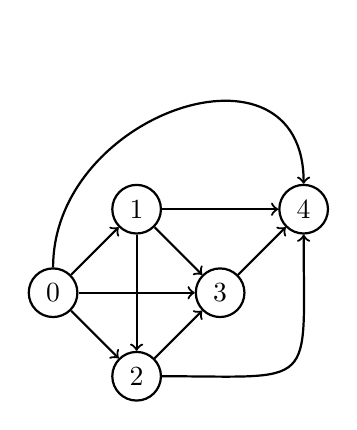
\begin{tikzpicture}[node distance={15mm}, thick, main/.style = {draw, circle}] 
        \node[main] (1) {$0$}; 
        \node[main] (2) [above right of=1] {$1$}; 
        \node[main] (3) [below right of=1] {$2$}; 
        \node[main] (4) [above right of=3] {$3$}; 
        \node[main] (5) [above right of=4] {$4$}; 
        \draw[->] (1) -- (2); 
        \draw[->] (1) -- (3); 
        \draw[->] (1) -- (4); 
        \draw[->] (1) to [out=90,in=90,looseness=1.5] (5); 
        \draw[->] (2) -- (3); 
        \draw[->] (2) -- (4); 
        \draw[->] (2) -- (5); 
        \draw[->] (3) -- (4); 
        \draw[->] (3) to [out=0, in=270,looseness=2] (5); 
        \draw[->] (4) -- (5); 
        \end{tikzpicture} 
  \end{center}
  textbfhe graph should be directed.
  \item Let $X = \{0, 1, 2, 3, 4\}$. Define a relation R on X such that $x R y$ if $x + y = 4$. Draw the graph associated with this relation. Should this graph be directed or undirected?
  \begin{center}
    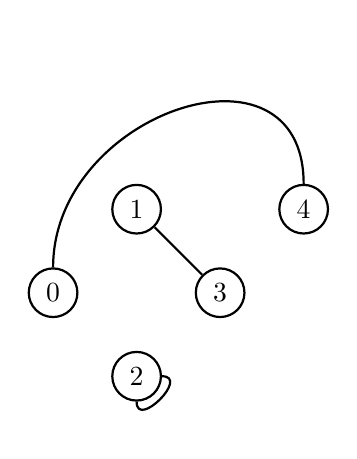
\begin{tikzpicture}[node distance={15mm}, thick, main/.style = {draw, circle}] 
        \node[main] (1) {$0$}; 
        \node[main] (2) [above right of=1] {$1$}; 
        \node[main] (3) [below right of=1] {$2$}; 
        \node[main] (4) [above right of=3] {$3$}; 
        \node[main] (5) [above right of=4] {$4$}; 
        \draw (1) to [out=90,in=90,looseness=1.5] (5);
        \draw (2) -- (4);
        \draw (3) to [out=0, in=270, looseness=2] (3);
        \end{tikzpicture} 
  \end{center}
  The graph should be undirected.
  \newpage
  For Exercises $3–6$, define a relation $\rightleftharpoons$ on the set S of all strings of letters: two strings are related if you can get one from the other by reversing one pair of adjacent letters. For example, $cow \rightleftharpoons ocw$ but $cow \text{~} \cancel{\rightleftharpoons} \text{~} woc$.
  \item Consider all the strings you can form with the letters c, a, and t (there are six). Draw the graph whose nodes are these six strings and whose edges represent the $\rightleftharpoons$ relation. Should this be a directed or an undirected graph?
  \begin{center}
    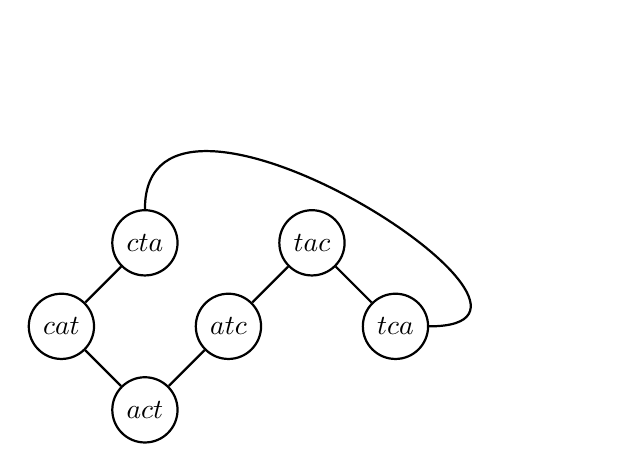
\begin{tikzpicture}[node distance={15mm}, thick, main/.style = {draw, circle}] 
        \node[main] (1) {$cat$}; 
        \node[main] (2) [above right of=1] {$cta$}; 
        \node[main] (3) [below right of=1] {$act$}; 
        \node[main] (4) [above right of=3] {$atc$}; 
        \node[main] (5) [above right of=4] {$tac$};
        \node[main] (6) [below right of=5] {$tca$}; 
        \draw(1) -- (3);
        \draw(1) -- (2);
        \draw(3) -- (4);
        \draw(4) -- (5);
        \draw(5) -- (6);
        \draw (2) to [out=90,in=0,looseness=1.5] (6);
        \end{tikzpicture} 
  \end{center}
  This should be an undirected graph.
  \item Find an Euler path in the graph you made in Exercise 3.\\
  The Euler path from the graph in Exercise 3 is: 
  \[cta \rightarrow cat \rightarrow act \rightarrow atc \rightarrow tac \rightarrow tca \rightarrow cta\]
  \item Consider the graph formed by the $\rightleftharpoons$ relation on the set of all the strings you can form from the letters l, y, n, and x. Does this graph have an Euler path? Why or why not?\\
  From the letters l, y, n and x, I can construct 24 strings. Each of those will have 3 possibilities to form a new string by reversing a pair of adjacent letters. \\
  Hence, each of the 24 vertices had an odd degree of 3 edges.\\
  Therefore, the graph does not have a Euler Path.
  \item Does the graph of the $\rightleftharpoons$ relation on the set of all strings formed from the letters l, e, o, p, a, r, and d have an Euler path? Why or why not?\\
  The number of string we can construct from the letters l, e, o, p, a, r and d is 5040 strings. Each of them has 6 possibilities to form a new string.\\
  Hence, the graph does have a Euler Path since they only have an even degree of 6 edges.
  \item Suppose you wanted to model an equivalence relation with a graph. Would you use a directed or an undirected graph? What would the equivalence classes look like? Explain.\\
  Because the relation is symmetric $((a \sim b) \rightarrow (b \sim a))$, the graph would be an undirected graph. \\
  The equivalence classes are represented by connected components because all elements in equivalence relation within the same class are related to each other. In a graph, this is modeled as a connected component, where every vertex is connected to every other vertex. 
  \item The “$\equiv \text{ mod } 3$” relation is an equivalence relation on the set {1, 2, 3, 4, 5, 6, 7}. List the equivalence classes.\\
  The equivalence classes are:
  \[[0] = \{3,6\}\]
  \[[1] = \{1,4,7\}\]
  \[[2] = \{2,5\}\]
  \item Define a relation on Z by $aRb$ if $a^2 = b^2$.
  \begin{enumerate}
    \item Prove that R is an equivalence relation.\\
    \textbf{Reflexive Proof}\\
    Let $a = b \text{ } \forall a,b \in Z$:
    \[\text{Clearly }a^2 = b^2\]
    Hence, the relation is reflexive.\\
    \textbf{Symmetric Proof}\\
    Suppose $a^2 = b^2$, obviously that $b^2 = a^2$ as well.\\
    Hence, the relation is also symmetric.\\
    \textbf{Transitivity}\\
    If $a^2 = b^2$ and $b^2 = c^2$, $a^2 = c^2$. Hence, the relation is transitivity.\\
    Therefore, the relation is equivalence.
    \item Describe the equivalence classes.
        \[[a] = \{b \in Z| b^2 = a^2\}\]
  \end{enumerate}
  \item Define a relation on Z by setting $x R y$ if xy is even.
  \begin{enumerate}
    \item Give a counterexample to show that R is not reflexive.\\
    Consider x = 1:\\
    For the relation to be reflexive 1R1 must hold, meaning $1 \times 1 = 1$ should be even. But 1 is odd, hence the relation is not reflexive.
    \item Give a counterexample to show that R is not transitive.\\
    Let x = 2, y = 3, z = 1.\\
    $xRy$ because $2 \times 3 = 6$ is even.\\
    $xRz$ because $2 \times 1 = 2$ is even.\\
    But $y \times z = 3 \times 1 = 3$ is odd.\\
    Hence $xRy$ and $xRz$ but y doesn't relate to z.\\
    Hence, the relation is not transitive.
  \end{enumerate}
  \item Explain why the web linking relation in Example 2.36 is not an equivalence relation. (You only need to give one reason why it fails to be an equivalence relation.)\\
  For a website, it may not link to itself. Hence $x \in W$ but $x \not\sim x$ and the relation is not reflexive. \\
  Therefore, the relation is not an equivalence relation.
  \item Prove that the relation defined in Example 2.46 is an equivalence relation.\\
  For every words $w_1 \in W$, $w_1$ will always have the same initial as $w_1$. Hence, the relation is reflexive.\\
  For every words $w_1, w_2 \in W$, if $w_1$ has the same initial as $w_2$, $w_2$ will always have the same initial as $w_1$. Hence, the relation is symmetric.\\
  For every words $w_1, w_2, w_3 \in W$, if $w_1 R w_2$ and $w_2 R w_3$, then $w_1 R w_3$. Hence, the relation is transitive.\\
  Therefore, the relation is an equivalence relation.
  \item The following set R defines an equivalence relation on the set \{1, 2, 3\}, where $a R b$ means that $(a, b) \in R$.
  \[R = \{(1,1),(2,2),(3,3),(2,3),(3,2)\}\]
  What are the equivalence classes?
  \[[1] = \{x \in \{1,2,3\}| (1,x) \in R\} = \{1\}\]
  \[[2] = \{x \in \{1,2,3\}| (2,x) \in R\} = \{2,3\}\]
  \[[3] = \{x \in \{1,2,3\}| (3,x) \in R\} = \{3,2\}\]
  \item Give a specific reason why the following set R does not define an equivalence relation on the set \{1, 2, 3, 4\}.
  \[R = \{(1,1),(2,2),(3,3),(4,4),(2,3),(3,2),(2,4),(4,2)\}\]
  $(4,2) \in R$ and $(2,3) \in R$ but $(4,3) \not\in R$. Hence, the relation is not transitive.\\
  Therefore, the relation is not an equivalence relation.
  \item Explain why the relation R on \{0, 1, 2\} given by 
  \[R = \{(0,0),(1,1),(2,2),(0,1),(1,0),(1,2),(2,1)\}\]
  is not an equivalence relation. Be specific.\\
  $(0,1) \in R$ and $(1,2) \in R$ but $(0,2) \not\in R$. Hence, the relation is not transitive.\\
  Therefore, the relation is not an equivalence relation.
  \item Let A = {1, 2}. Write out the subset of $A \times A$ defined by the $\leq$ relation on A.\\
  Let R is the relation $\leq$ on A.
  \[R = \{(1,1),(2,2),(1,2)\}\]
  \item Let $X = \{0,1\}$.
  \begin{enumerate}
    \item List (as subsets of $X \times X$) all possible relations on X.
        \[R_1 = X \times X = \{(0,0),(0,1),(1,0),(1,1)\}\]
        \[R_2 = \{(0,0),(0,1),(1,0)\}\]
        \[R_3 = \{(0,0),(0,1),(1,1)\}\]
        \[R_4 = \{(0,0),(1,0),(1,1)\}\]
        \[R_5 = \{(0,1),(1,0),(1,1)\}\]
        \[R_6 = \{(0,0),(0,1)\}\]
        \[R_7 = \{(1,0),(1,1)\}\]
        \[R_8 = \{(0,0),(1,0)\}\]
        \[R_9 = \{(0,1),(1,1)\}\]
        \[R_{10} = \{(0,1),(1,0)\}\]
        \[R_{11} = \{(0,0),(1,1)\}\]
        \[R_{12} = \{(0,0)\}\]
        \[R_{13} = \{(0,1)\}\]
        \[R_{14} = \{(1,0)\}\]
        \[R_{15} = \{(1,1)\}\]
        \[R_{16} = \emptyset\]
    \item Which of the relations in part (a) are equivalence relations?\\
    The relation $R_1 = \{(0,0),(0,1),(1,0),(1,1)\}$, and $R_{11} = \{(0,0),(1,1)\}$ are the equivalence relations.
  \end{enumerate}
  \item Let X be a nonempty set. Define a relation R on the power set P(X) by
  \[ARB \leftrightarrow A\cap B = \emptyset\]
  for $A, B \in (X)$. Determine whether this relation is reflexive, symmetric, and/or transitive.\\
  The relation is not reflexive because for $A \in X$, $A \cap A = A$ and $A \not\sim A$. \\
  The relation is symmetric because for $A,B \in X$, if $A \cap B = \emptyset$ then $B \cap A = \emptyset$.\\
  The relation is not transitive because for $A,B,C \in X$ with A = C, if $A \cap B = \emptyset$ and $B \cap C = \emptyset$ but $A \cap C = A \text{ or } A \cap C = C$. Hence $A \sim B$, $B\sim C$ but $A \not\sim C$.


\end{enumerate}
\end{document}